\documentclass[journal,12pt,twocolumn]{IEEEtran}

\usepackage{enumitem}
\usepackage{amsmath}
\usepackage{amssymb}
\usepackage{gensymb}
\usepackage{graphicx}
\usepackage{txfonts}         
\usepackage{listings}
\usepackage{lstautogobble}
\usepackage{mathtools}
\usepackage{bm}
\usepackage{hyperref}
\usepackage{polynom}
\usepackage{siunitx}
\usepackage{verbatim}
\usepackage[siunitx]{circuitikz}

\newcommand{\solution}{\noindent \textbf{Solution: }}
\providecommand{\pr}[1]{\ensuremath{\Pr\left(#1\right)}}
\providecommand{\brak}[1]{\ensuremath{\left(#1\right)}}
\providecommand{\cbrak}[1]{\ensuremath{\left\{#1\right\}}}
\providecommand{\sbrak}[1]{\ensuremath{\left[#1\right]}}
\providecommand{\mean}[1]{E\left[ #1 \right]}
\providecommand{\var}[1]{\mathrm{Var}\left[ #1 \right]}
\providecommand{\der}[1]{\mathrm{d} #1}
\providecommand{\gauss}[2]{\mathcal{N}\ensuremath{\left(#1,#2\right)}}
\providecommand{\mbf}{\mathbf}
\providecommand{\abs}[1]{\left\vert#1\right\vert}
\providecommand{\norm}[1]{\left\lVert#1\right\rVert}
\providecommand{\z}[1]{{\mathcal{Z}}\cbrak{#1}}
\providecommand{\ztrans}{\overset{\mathcal{Z}}{ \rightleftharpoons}}
\providecommand{\system}[1]{\overset{\mathcal{#1}}{ \longleftrightarrow}}
\providecommand{\parder}[2]{\frac{\partial}{\partial #2} \brak{#1}}

\let\StandardTheFigure\thefigure
\let\vec\mathbf

\numberwithin{equation}{section}
\numberwithin{figure}{section}
\renewcommand{\thefigure}{\theenumi}
\renewcommand\thesection{\arabic{section}}

\newcommand{\myvec}[1]{\ensuremath{\begin{pmatrix}#1\end{pmatrix}}}
\newcommand{\mymat}[1]{\ensuremath{\begin{bmatrix}#1\end{bmatrix}}}
\newcommand{\mydet}[1]{\ensuremath{\begin{vmatrix}#1\end{vmatrix}}}
\newcommand{\define}{\stackrel{\triangle}{=}}

\DeclareMathOperator*{\argmin}{arg\,min}
\DeclareMathOperator*{\argmax}{arg\,max}

\makeatletter
\def\pld@CF@loop#1+{%
    \ifx\relax#1\else
        \begingroup
          \pld@AccuSetX11%
          \def\pld@frac{{}{}}\let\pld@symbols\@empty\let\pld@vars\@empty
          \pld@false
          #1%
          \let\pld@temp\@empty
          \pld@AccuIfOne{}{\pld@AccuGet\pld@temp
                            \edef\pld@temp{\noexpand\pld@R\pld@temp}}%
           \pld@if \pld@Extend\pld@temp{\expandafter\pld@F\pld@frac}\fi
           \expandafter\pld@CF@loop@\pld@symbols\relax\@empty
           \expandafter\pld@CF@loop@\pld@vars\relax\@empty
           \ifx\@empty\pld@temp
               \def\pld@temp{\pld@R11}%
           \fi
          \global\let\@gtempa\pld@temp
        \endgroup
        \ifx\@empty\@gtempa\else
            \pld@ExtendPoly\pld@tempoly\@gtempa
        \fi
        \expandafter\pld@CF@loop
    \fi}
\def\pld@CMAddToTempoly{%
    \pld@AccuGet\pld@temp\edef\pld@temp{\noexpand\pld@R\pld@temp}%
    \pld@CondenseMonomials\pld@false\pld@symbols
    \ifx\pld@symbols\@empty \else
        \pld@ExtendPoly\pld@temp\pld@symbols
    \fi
    \ifx\pld@temp\@empty \else
        \pld@if
            \expandafter\pld@IfSum\expandafter{\pld@temp}%
                {\expandafter\def\expandafter\pld@temp\expandafter
                    {\expandafter\pld@F\expandafter{\pld@temp}{}}}%
                {}%
        \fi
        \pld@ExtendPoly\pld@tempoly\pld@temp
        \pld@Extend\pld@tempoly{\pld@monom}%
    \fi}
\makeatother

\lstset {
	frame=single, 
	breaklines=true,
	columns=fullflexible,
	autogobble=true
}             
                               
\title{Circuits and Transforms \\ \Large EE3900 - Linear Systems and Signal Processing \\ \large IIT Hyderabad}
\author{Adithya Ram Malothu \\ \normalsize BM20BTECH11009 \\ \vspace*{20pt} \normalsize 13TH Oct 2022}

\begin{document}

	\maketitle

	\section{Definitions}
	\begin{enumerate}[label=\thesection.\arabic*,ref=\thesection.\theenumi]
	\item The unit step function is defined as
	\begin{align}
		u(t) =
		\begin{cases}
			1 & t > 0 \\
			\frac{1}{2} & t = 0 \\
			0 & t < 0
		\end{cases}
	\end{align}
		
	\item The Laplace transform of $g(t)$ is defined as 
	\begin{align}
		G(s) = \int_{-\infty}^{\infty} g(t) e^{-st}\, \der{t}
	\end{align}
	\end{enumerate}
	
	\section{Laplace Transform}
	\begin{enumerate}[label=\thesection.\arabic*.,ref=\thesection.\theenumi]
	\item In the circuit, the switch S is connected to position P for a long time so that the charge on the capacitor becomes $q_1$ \SI{}{\micro\coulomb}. Then S is switched to position Q.  After a long time, the charge on the capacitor is $q_2$ \SI{}{\micro\coulomb}
	
	\item Draw the circuit using latex-tikz
	
	\solution
	\begin{figure}[!ht]
		\centering
		\begin{circuitikz} \draw
			(0,3) to[battery1, l_=1<\volt>] (0,0) -- (8,0)
			(8,3) to[battery1, l=2<\volt>] (8,0)
			(4,0) to[C=1<\micro\farad>] (4,3)
				to[R=$2\,\Omega$] (8,3)
			(4,3) to[R, l_=$1\,\Omega$] (1,3)
				to[nos, l_=S, mirror] (0,3) node[label={left:P}]{}
			(0.7,0) -- (0.7,2.7) node[label={right:Q}]{}
			;
		\end{circuitikz}
		\caption{Circuit diagram of the circuit in question}
		\label{fig:ckt}
	\end{figure}
	
	\item Find $q_1$
	
	\solution After a long time, when steady state is achieved, a capacitor behaves like an open circuit, i.e., current passing through it is zero
	\begin{figure}[!ht]
		\centering
		\begin{circuitikz} \draw
			(0,3) to[battery1, l_=1<\volt>] (0,0) node[label={below:0}]{} 
				-- (8,0) node[label={below:0}]{}
			(8,3) node[label={above:2}]{} to[battery1, l=2<\volt>] (8,0)
			(4,3) node[label={above:$V$}] {} to[R=$2\,\Omega$] (8,3)
			(4,3) to[R, l_=$1\,\Omega$] (0,3) node[label={above:1}]{}
			(4,0) node[ground]{}
			;
		\end{circuitikz}
		\caption{Circuit diagram at steady state before flipping the switch}
	\end{figure}
	
	By Kirchoff's junction law, we get
	\begin{align}
		\frac{V - 1}{1} &+ \frac{V - 2}{2} = 0 \\
		\implies V &= \SI[parse-numbers=false]{\frac{4}{3}}{\volt} \\
		\implies q_1 &= CV = \SI[parse-numbers=false]{\frac{4}{3}}{\micro\coulomb}
	\end{align}
	
	\item Show that the Laplace transform of $u(t)$ is $\frac{1}{s}$ and find the ROC
	
	\solution The Laplace transform of $u(t)$ is given by
	\begin{align}
    		\mathcal{L}\cbrak{u(t)} &=\int_{-\infty}^{\infty}u(t)e^{-st} \,\der{t} \\
        &= \int_{0}^{\infty}e^{-st} \,\der{t} \\
        &= \lim_{R \to \infty} \frac{1 - e^{-sR}}{s}
	\end{align}
	
	This limit is finite only if $\Re(s) > 0$, which is going to be its ROC
	
	Therefore
	\begin{align}
		u(t) \system{L} \frac{1}{s} \qquad \Re(s) > 0
	\end{align}
	
	\item Show that 
	\begin{align}
		e^{-at}u(t) \system{L} \frac{1}{s+a} \qquad a > 0
	\end{align}
	and find the ROC
	
	\solution The Laplace transform of $e^{-at}u(t)$ for $a>0$ is given by
	\begin{align}
    		\mathcal{L}\cbrak{u(t)} &=\int_{-\infty}^{\infty}e^{-at}u(t)e^{-st} \,\der{t} \\
        &= \int_{0}^{\infty}e^{-(s+a)t} \,\der{t} \\
        &= \lim_{R \to \infty} \frac{1 - e^{-(s+a)R}}{s+a}
	\end{align}	
	
	This limit is finite only if $\Re(s + a) > 0$, which is going to be its ROC
	
	Therefore
	\begin{align}
		e^{-at}u(t) \system{L} \frac{1}{s+a} \qquad \Re(s) > -a
	\end{align}
	since $a$ is real
	
	\item Now consider the following resistive circuit transformed from Fig. \ref{fig:ckt}
	\begin{figure}[!ht]
		\centering
		\begin{circuitikz} \draw
			(0,3) to[battery1, l_=$V_1(s)$] (0,0) node[label={below:0}]{} 
				-- (6,0) node[label={below:0}]{}
			(6,3) node[label={above:$V_2$}]{} to[battery1, l_=$V_2(s)$] (6,0)
			(3,3) node[label={above:$V_c(s)$}] {} to[generic, l=$R_2$] (6,3)
			(3,3) to[generic, l_=$R_1$] (0,3) node[label={above:$V_1$}]{}
			(3,0) node[ground]{} to[generic, l=$\frac{1}{sC_0}$] (3,3)
			;
		\end{circuitikz}
		\caption{Circuit diagram in $s$-domain before flipping the switch}
		\label{fig:lap}
	\end{figure}
		
	where 
	\begin{align}
		u(t) \system{L} V_1(s) \\
		2u(t) \system{L} V_2(s)
	\end{align}
	Find the voltage across the capacitor $V_c(s)$
	
	\solution 
	\begin{align}
		V_1(s) &= \frac{1}{s} &&\Re(s) > 0 \\
		V_2(s) &= \frac{2}{s} &&\Re(s) > 0 
	\end{align}		
		
	By Kirchoff's junction law, we get
	\begin{align}
		&\frac{V_c - V_1}{R_1} + 	\frac{V_c - V_2}{R_2} + \frac{V_c - 0}{\frac{1}{sC_0}} = 0 \\
		\implies &V_c \brak{\frac{1}{R_1} + \frac{1}{R_2} + sC_0} = \frac{V_1}{R_1} + \frac{V_2}{R_2} \\
		\implies &V_c(s) = \frac{\frac{1}{sR_1} + \frac{2}{sR_2}}{\frac{1}{R_1} + \frac{1}{R_2} + sC_0} \\
		&\qquad = \frac{\frac{1}{R_1C_0} + \frac{2}{R_2C_0}}{s\brak{s + \frac{1}{R_1C_0} + \frac{1}{R_2C_0}}} 
	\end{align}
	
	\item Find $v_c(t)$. Plot using Python.

	\solution On performing partial fraction decomposition
	\begin{align} 
		V_c(s) &=  \frac{\frac{1}{R_1C_0} + \frac{2}{R_2C_0}}{\frac{1}{R_1C_0} + \frac{1}{R_2C_0}} \brak{\frac{1}{s} - \frac{1}{s + \frac{1}{R_1C_0} + \frac{1}{R_2C_0}}}, \Re(s) > 0
	\end{align}
	
	On taking the inverse Laplace transform, we get
	\begin{align}
	v_c(t) &= \frac{2R_1 + R_2}{R_1 + R_2} \brak{u(t) - e^{-\brak{\frac{1}{R_1} + \frac{1}{R_2}} \frac{t}{C_0}} u(t)} \\
	&= \frac{2R_1 + R_2}{R_1 + R_2} \brak{1 - e^{-\brak{\frac{1}{R_1} + \frac{1}{R_2}} \frac{t}{C_0}} }u(t)
	\end{align}
	
	Substitute the values $R_1 = \SI{1}{\ohm}, R_2 = \SI{2}{\ohm}, C_0 = \SI{1}{\micro\farad}$
	\begin{align}
		v_c(t) = \SI[parse-numbers=false]{\frac{4}{3} \brak{1 - e^{-\frac{3}{2} \times 10^6 t}} u(t)}{\volt}
	\end{align}
	
	\item Verify your result using ngspice
	
	\solution Download the following codes for simulation and plotting Fig. \ref{fig-2} respectively
	\begin{lstlisting}
		wget https://github.com/adithyajadhav01/EE3900/blob/main/CIRCUITS/codes/2.8.cir
		wget https://github.com/adithyajadhav01/EE3900/blob/main/CIRCUITS/codes/2.7.py
	\end{lstlisting}
	
	Run the codes by executing
	\begin{lstlisting}
		ngspice 2.8.cir
		python 2.7.py
	\end{lstlisting}	
	
	\begin{figure}[!ht]
		\centering
		\includegraphics[width=\columnwidth]{./figures/2.png}
		\caption{Plot of $v_c(t)$ before flipping the switch}
		\label{fig-2}	
	\end{figure}
	
	\item Obtain Fig. \ref{fig:lap} using the equivalent differential equation
	
	\solution Using Kirchoff's junction law
	\begin{align}
		\frac{v_c(t) - v_1(t)}{R_1} + \frac{v_c(t) - v_2(t)}{R_2} + \frac{\der{q}}{\der{t}} = 0
	\end{align}
	where $q(t)$ is the charge on the capacitor
	
	On taking the Laplace transform on both sides of this equation
	\begin{align}
		\frac{V_c(s) - V_1(s)}{R_1} + \frac{V_c(s) - V_2(s)}{R_2} + \brak{sQ(s) - q(0^-)} = 0
	\end{align}
	
	But $q(0^-) = 0$ and 
	\begin{align}
		q(t) &= C_0v_c(t) \\
		\implies Q(s) &= C_0V_c(s)
	\end{align}
	
	Thus
	\begin{align}
		&\frac{V_c(s) - V_1(s)}{R_1} + \frac{V_c(s) - V_2(s)}{R_2} + sC_0V_c(s) = 0 \\
		\implies &\frac{V_c(s) - V_1(s)}{R_1} + 	\frac{V_c(s) - V_2(s)}{R_2} + \frac{V_c(s) - 0}{\frac{1}{sC_0}} = 0 
	\end{align}
	
	which is the same equation as the one we obtained from Fig. \ref{fig:lap}
	
	\end{enumerate}
	
	
	\section{Initial Conditions}
	\begin{enumerate}[label=\thesection.\arabic*.,ref=\thesection.\theenumi]
	\item Find $q_2$ in Fig. \ref{fig:ckt}
	
	\solution After a long time, when steady state is achieved, a capacitor behaves like an open circuit, i.e., current passing through it is zero
	
	\begin{figure}[!ht]
		\centering
		\begin{circuitikz} \draw
			(0,3) -- (0,0) node[label={below:0}]{} 
				-- (8,0) node[label={below:0}]{}
			(8,3) node[label={above:2}]{} to[battery1, l=2<\volt>] (8,0)
			(4,3) node[label={above:$V$}] {} to[R=$2\,\Omega$] (8,3)
			(4,3) to[R, l_=$1\,\Omega$] (0,3) node[label={above:0}]{}
			(4,0) node[ground]{}
			;
		\end{circuitikz}
		\caption{Circuit diagram at steady state after flipping the switch}
	\end{figure}
	
	By Kirchoff's junction law, we get
	\begin{align}
		\frac{V - 0}{1} &+ \frac{V-2}{2} = 0 \\
		\implies V &= \SI[parse-numbers=false]{\frac{2}{3}}{\volt} \\
		\implies q_2 &= CV = \SI[parse-numbers=false]{\frac{2}{3}}{\micro\coulomb}
	\end{align}
	
	\item Draw the equivalent $s$-domain resistive circuit when S is switched to position Q.  Use variables $R_1, R_2, C_0$ for the passive elements.
Use latex-tikz

	\solution
	\begin{figure}[!ht]
		\centering
		\begin{circuitikz} \draw
			(0,3) -- (0,0) node[label={below:0}]{} 
				-- (6,0) node[label={below:0}]{}
			(6,3) node[label={above:$V_2$}]{} to[battery1, l_=$V_2(s)$] (6,0)
			(3,3) node[label={above:$V_c(s)$}] {} to[generic, l=$R_2$] (6,3)
			(3,3) to[generic, l_=$R_1$] (0,3) node[label={above:0}]{}
			(3,1) to[battery1, l=$\frac{4}{3s}$] (3,0) node[ground]{}
			(3,1) to[generic, l=$\frac{1}{sC_0}$] (3,3)
			;
		\end{circuitikz}
		\caption{Circuit diagram in $s$-domain after flipping the switch}
		\label{prob:init}
	\end{figure}
	
	The battery $\frac{4}{3s}$ corresponds to the intial potential difference of $\SI[parse-numbers=false]{\frac43}{\volt}$ across the capacitor just before switching it to Q
	
	\item Find $V_c(s)$
	
	\solution 
	By Kirchoff's junction law, we get
	\begin{align}
		&\frac{V_c - 0}{R_1} + 	\frac{V_c - V_2}{R_2} + \frac{V_c - \frac{4}{3s}}{\frac{1}{sC_0}} = 0 \\
		\implies &V_c \brak{\frac{1}{R_1} + \frac{1}{R_2} + sC_0} =  \frac{V_2}{R_2} + \frac{4}{3}C_0 \\
		\implies &V_c(s) = \frac{\frac{2}{sR_2} + \frac{4}{3}C_0}{\frac{1}{R_1} + \frac{1}{R_2} + sC_0} \\
		&\qquad = \frac{\frac{2}{R_2C_0} + \frac43 s}{s\brak{s + \frac{1}{R_1C_0} + \frac{1}{R_2C_0}}} 
	\end{align}
	
	\item Find $v_c(t)$. Plot using Python
	
	\solution On performing partial fraction decomposition
	\begin{multline}
    V_{c}(s) = \frac{4}{3}\brak{\frac{1}{s + \frac{1}{R_1C_0} + \frac{1}{R_2C_0}}} \\
    + \frac{\frac{2}{R_2C_0}}{\frac{1}{R_1C_0} +\frac{1}{R_2C_0}}\brak{\frac{1}{s} - \frac{1}{s + \frac{1}{R_1C_0} + \frac{1}{R_2C_0}}} 
	\end{multline}
	for $\Re(s) > 0$
	
	On taking the inverse Laplace transform, we get
	\begin{multline}
    v_c(t) = \frac{4}{3}e^{-\brak{\frac{1}{R_1} + \frac{1}{R_2}}\frac{t}{C_0}}u(t) \\
    + \frac{2R_1}{R_1 + R_2} \brak{u(t) - e^{-\brak{\frac{1}{R_1} + \frac{1}{R_2}}\frac{t}{C_0}}u(t) } 
	\end{multline}
	
	Substitute the values $R_1 = \SI{1}{\ohm}, R_2 = \SI{2}{\ohm}, C_0 = \SI{1}{\micro\farad}$
	\begin{align}
		v_c(t) &= \frac43 e^{-\frac{3}{2} \times 10^6 t}u(t) + \frac{2}{3}\brak{1 - e^{-\frac{3}{2} \times 10^6 t}}u(t) \\
		&= \SI[parse-numbers=false]{\frac{2}{3} \brak{1 + e^{-\frac{3}{2} \times 10^6 t}} u(t)}{\volt}
	\end{align}
	
	\item Verify your result using ngspice
	
	\solution Download the following codes for simulation and plotting Fig. \ref{fig-3} respectively
	\begin{lstlisting}
		wget https://github.com/adithyajadhav01/EE3900/blob/main/CIRCUITS/codes/3.5.cir
		wget https://github.com/adithyajadhav01/EE3900/blob/main/CIRCUITS/codes/3.4.py
	\end{lstlisting}
	
	Run the codes by executing
	\begin{lstlisting}
		ngspice 3.5.cir
		python 3.4.py
	\end{lstlisting}	
	
	\begin{figure}[!ht]
		\centering
		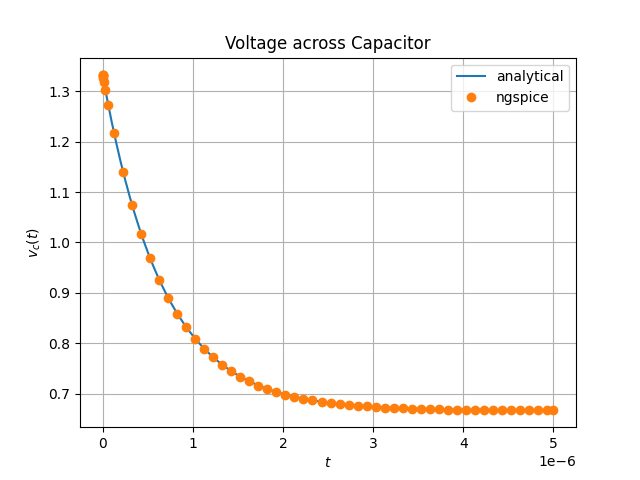
\includegraphics[width=\columnwidth]{./figures/3.png}
		\caption{Plot of $v_c(t)$ after flipping the switch}
		\label{fig-3}	
	\end{figure}
	
	\item Find $v_c(0^-)$, $v_c(0^+)$ and $v_c(\infty)$
	
	\solution At $t = 0^-$, the switch still hasn't been switched to Q and the circuit is in steady state
	\begin{align}
		v_c(0^-) = \SI[parse-numbers=false]{\frac43}{\volt}
	\end{align}
	
	For $t \ge 0$, we can use the above formula
	\begin{align}
		v_c(0^+) &= \lim_{t\to0^+}v_c(t) = \SI[parse-numbers=false]{\frac43}{\volt} \\
		v_c(\infty) &= \lim_{t\to\infty}v_c(t) = \SI[parse-numbers=false]{\frac23}{\volt}
	\end{align}
	
	\item Obtain Fig. \ref{prob:init} using the equivalent differential equation
	
	\solution Using Kirchoff's junction law
	\begin{align}
		\frac{v_c(t) - 0}{R_1} + \frac{v_c(t) - v_2(t)}{R_2} + \frac{\der{q}}{\der{t}} = 0
	\end{align}
	where $q(t)$ is the charge on the capacitor
	
	On taking the Laplace transform on both sides of this equation
	\begin{align}
		\frac{V_c(s) - 0}{R_1} + \frac{V_c(s) - V_2(s)}{R_2} + \brak{sQ(s) - q(0^-)} = 0
	\end{align}
	
	But $q(0^-) = \frac43 C_0$ and 
	\begin{align}
		q(t) &= C_0v_c(t) \\
		\implies Q(s) &= C_0V_c(s)
	\end{align}
	
	Thus
	\begin{align}
		&\frac{V_c(s) - 0}{R_1} + \frac{V_c(s) - V_2(s)}{R_2} + \brak{sC_0V_c(s) - \frac43 C_0} = 0 \\
		\implies &\frac{V_c(s) - 0}{R_1} + 	\frac{V_c(s) - V_2(s)}{R_2} + \frac{V_c(s) - \frac{4}{3s}}{\frac{1}{sC_0}} = 0 
	\end{align}
	
	which is the same equation as the one we obtained from Fig. \ref{prob:init}
	\end{enumerate}

	\section{Bilinear Transform}
	\begin{enumerate}[label=\thesection.\arabic*.,ref=\thesection.\theenumi]
	\item In Fig. \ref{fig:ckt}, consider the case when $S$ is switched to $Q$ right in the beginning. Formulate the differential equation
	
	\solution The differential equation is the same as before 
	\begin{align}
		&\frac{v_c(t) - 0}{R_1} + \frac{v_c(t) - v_2(t)}{R_2} + \frac{\der{q}}{\der{t}} = 0 \\
		\text{i.e., } &\frac{v_c(t)}{R_1} + \frac{v_c(t) - v_2(t)}{R_2} + C_0\frac{\der{v_c}}{\der{t}} = 0
	\end{align}
	
	but with a different initial condition
	\begin{equation}
		q(0^-) = q(0) = 0
	\end{equation}
	
	\item Find $H(s)$ considering the ouput voltage at the capacitor
	
	\solution On taking the Laplace transform on both sides of this equation
	\begin{align}
		&\frac{V_c(s)}{R_1} + \frac{V_c(s) - V_2(s)}{R_2} + sQ(s) - 0 = 0 \\
		\implies &V_c(s) \brak{\frac{1}{R_1} + \frac{1}{R_2}} + sC_0V_c(s) = \frac{V_2(s)}{R_2} \\
		\implies &\frac{V_c(s)}{V_2(s)} = \frac{\frac{1}{R_2}}{\frac{1}{R_1} + \frac{1}{R_2} + sC_0}
	\end{align}
	
	The transfer function is thus
	\begin{align}
		H(s) = \frac{\frac{1}{R_2C_0}}{s + \frac{1}{R_1C_0} + \frac{1}{R_2C_0}}
	\end{align}
	
	On substituting the values, we get
	\begin{equation}
		H(s) = \frac{5 \times 10^5}{s + 1.5 \times 10^6}
	\end{equation}
	
	\item Plot $H(s)$.  What kind of filter is it?
	
	\solution Download the following Python code that plots Fig. \ref{fig-4.3}
	\begin{lstlisting}
		wget https://github.com/adithyajadhav01/EE3900/blob/main/CIRCUITS/codes/4.3.py
	\end{lstlisting}
	
	Run the codes by executing
	\begin{lstlisting}
		python 4.3.py
	\end{lstlisting}	
	
	\begin{figure}[!ht]
		\centering
		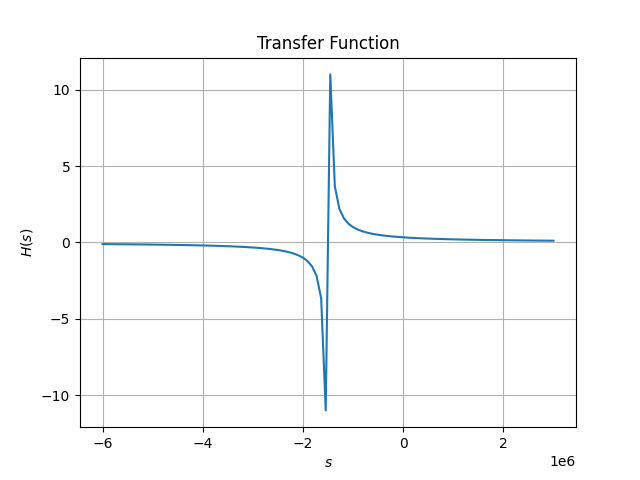
\includegraphics[width=\columnwidth]{./figures/4.3.png}
		\caption{Plot of $H(s)$}
		\label{fig-4.3}	
	\end{figure}
	
	Consider the frequency-domain transfer function by putting $s = \j\omega$
	\begin{align}
		H(\j\omega) &= \frac{5 \times 10^5}{\j\omega + 1.5 \times 10^6} \\
		\implies \abs{H(\j\omega)} &= \frac{5 \times 10^5}{\sqrt{\omega^2 + 2.25\times10^{12}}}
	\end{align}
	
	As $\omega$ increases, $\abs{H(\j\omega)}$ decreases
	
	In other words, the amplitude of high-frequency signals gets diminished and they get filtered out
	
	Therefore, this is a low-pass filter
	
	\item Using trapezoidal rule for integration, formulate the difference equation by considering 
	\begin{align}
		y(n) = y(t)\vert_{t=n}
	\end{align}
	
	\solution
	\begin{align}
		&\frac{v_c(t)}{R_1} + \frac{v_c(t) - v_2(t)}{R_2} + C_0\frac{\der{v_c}}{\der{t}} = 0 \\
		\implies &C_0\frac{\der{v_c}}{\der{t}} = \frac{2u(t)-v_c(t)}{R_2} - \frac{v_c(t)}{R_1} \\
		\implies &\left.v_c(t)\right|_{t=n}^{n+1} = \int_{n}^{n+1} \brak{\frac{2u(t)-v_c(t)}{R_2C_0} - \frac{v_c(t)}{R_1C_0}} \der{t}
	\end{align}
	
	By the trapezoidal rule of integration
	\begin{align}
		\int_a^b f(t) \der{t} \approx \frac{b-a}{2} (f(a) + f(b))
	\end{align}
	
	Consider $y(t) = v_c(t)$
	\begin{multline}
		y(n+1) - y(n) = \frac{1}{R_2C_0}\brak{u(n)+u(n+1)} \\
		- \frac12(y(n+1) + y(n))\brak{\frac{1}{R_1C_0} + \frac{1}{R_2C_0}}
	\end{multline}
	
	Thus, the difference equation is
	\begin{multline}
		y(n+1) \brak{1 + \frac{1}{2R_1C_0} + \frac{1}{2R_2C_0}} \\= y(n) \brak{1 - \frac{1}{2R_1C_0} - \frac{1}{2R_2C_0}} \\+ \frac{1}{R_2C_0}\brak{u(n)+u(n+1)}
	\end{multline}
	
	\item Find $H(z)$
	
	\solution Let $\z{y(n)} = Y(z)$
	
	On taking the $Z$-transform on both sides of the difference equation
	\begin{multline}
		zY(z)\brak{1 + \frac{1}{2R_1C_0} + \frac{1}{2R_2C_0}} \\= Y(z)\brak{1 - \frac{1}{2R_1C_0} - \frac{1}{2R_2C_0}} \\+ \frac{1}{R_2C_0} \brak{\frac{1}{1-z^{-1}} + \frac{z}{1-z^{-1}}}
	\end{multline}
	\begin{multline}
		Y(z)\brak{z + \frac{z}{2R_1C_0} + \frac{z}{2R_2C_0} - 1 + \frac{1}{2R_1C_0} + \frac{1}{2R_2C_0}} \\
		= \frac{1}{R_2C_0} \frac{1+z}{1-z^{-1}}
	\end{multline}
	
	Also
	\begin{align}
		v_2(t) &= 2 &&\forall t \ge 0\\
		\implies x(n) &= 2u(n) \\
		\implies X(z) &= \frac{2}{1-z^{-1}} &&\abs{z} > 1
	\end{align}
	
	Thus, the transfer function in $z$-domain is
	\begin{align}
		H(z) &= \frac{Y(z)}{X(z)} \\
		&= \frac{\frac{1+z}{2R_2C_0}}{z + \frac{z}{2R_1C_0} + \frac{z}{2R_2C_0} - 1 + \frac{1}{2R_1C_0} + \frac{1}{2R_2C_0}} \\
		&= \frac{\frac{1 + z^{-1}}{2R_2C_0}}{1 + \frac{1}{2R_1C_0} + \frac{1}{2R_2C_0} - z^{-1} + \frac{z^{-1}}{2R_1C_0} + \frac{z^{-1}}{2R_2C_0}}
	\end{align}
	
	On substituting the values
	\begin{align}
		H(z) &= \frac{2.5\times10^5 (1+z^{-1})}{7.5\times10^5 + 1 + (7.5\times10^5 - 1)z^{-1}}
	\end{align}
	
	with the ROC being
	\begin{align}
		\abs{z} &> \max\brak{1, \abs{\frac{7.5\times10^5 - 1}{7.5\times10^5 + 1}}} \\
		\implies \abs{z} &> 1
	\end{align}
	
	\item How can you obtain $H(z)$ from $H(s)$?
	
	\solution The $Z$-transform can be obtained from the Laplace transform by the substitution
	\begin{align}
		s &= \frac{2}{T} \frac{1-z^{-1}}{1+z^{-1}}
	\end{align}
	where $T$ is the step size of the trapezoidal rule ($1$ in our case)
	
	This is known as the bilinear transform
	
	Thus
	\begin{align}
		H(z) &= \frac{\frac{1}{R_2C_0}}{2\frac{1-z^{-1}}{1+z^{-1}} + \frac{1}{R_1C_0} + \frac{1}{R_2C_0}} \\
		&= \frac{\frac{1 + z^{-1}}{2R_2C_0}}{1-z^{-1}	 + \brak{\frac{1}{2R_1C_0} + \frac{1}{2R_2C_0}}(1 + z^{-1})} \\
		&= \frac{\frac{1 + z^{-1}}{2R_2C_0}}{1 + \frac{1}{2R_1C_0} + \frac{1}{2R_2C_0} - z^{-1} + \frac{z^{-1}}{2R_1C_0} + \frac{z^{-1}}{2R_2C_0}} \\
		&= \frac{2.5\times10^5 (1+z^{-1})}{7.5\times10^5 + 1 + (7.5\times10^5 - 1)z^{-1}}
	\end{align}
	which is the same as what we obtained earlier
	
	\item Find $y(n)$ from $H(z)$ and verify whether $y(n) = y(t)|_{t=n}$
	
	\solution 
	\begin{align}
		Y(z) &= H(z)X(z) \\
		&= \frac{2.5\times10^5 (1+z^{-1})}{7.5\times10^5 + 1 + (7.5\times10^5 - 1)z^{-1}} \frac{2}{1-z^{-1}} \\
		&= \frac{\frac{2}{3}}{1-z^{-1}} -\frac{\frac{2}{3}}{7.5\times10^5 + 1 + (7.5\times10^5 - 1)z^{-1}}
	\end{align}
	
	On taking the inverse $Z$-transform by considering the ROC to be $\abs{z} > 1$, we get
	\begin{align}
		y(n) &= \frac{2}{3}u(n) - \frac{2}{3}\brak{-\frac{7.5\times10^5 - 1}{7.5\times10^5 + 1}}^nu(n) \\
		&= \frac{2}{3} \brak{1 - \brak{\frac{1-7.5\times10^5}{1+7.5\times10^5}}^n}u(n)
	\end{align}
	
	If we are sampling the signal at intervals of $T \ll 10^{-5}$, say $\SI[parse-numbers=false]{10^{-7}}{\second}$, i.e., $n = 10^{-7}, 2\times10^{-7},\ldots$
	\begin{align}
		y(n) &\approx \frac{2}{3} \brak{1 - \frac{1-7.5\times10^5n}{1+7.5\times10^5n}}u(n)
	\end{align}
	
	Now
	\begin{align}
		Y(s) &= H(s)X(s) \\
		&= \frac{5\times10^5}{s+1.5\times10^6} \frac{2}{s} \\
		&= \frac{10^6}{1.5\times10^6} \brak{\frac{1}{s} - \frac{1}{s+1.5\times10^6}}
	\end{align}
	
	On taking the inverse Laplace transform by considering the ROC to be $\Re(s) > 0$, we get
	\begin{align}
		y(t) = \frac{2}{3}\brak{1 - e^{-1.5\times10^6t}}u(t)
	\end{align}
	
	But 
	\begin{align}
		e^{-1.5\times 10^6 t} &= \frac{e^{-0.75 \times 10^6 t}}{e^{0.75 \times 10^6 t}} \\
		&\approx \frac{1-7.5\times10^5t}{1+7.5\times10^5t} && \text{when } t \ll 10^{-6} 
	\end{align}
	
	Therefore
	\begin{align}
		y(t) &\approx \frac{2}{3} \brak{1 - \frac{1-7.5\times10^5t}{1+7.5\times10^5t}} u(t) \\
		\therefore y(n) &= y(t)|_{t=n}
	\end{align}
	
	Download the following codes for simulation and plotting Fig. \ref{fig-4.7} respectively
	\begin{lstlisting}
		wget https://github.com/adithyajadhav01/EE3900/blob/main/CIRCUITS/codes/4.7.cir
		wget https://github.com/adithyajadhav01/EE3900/blob/main/CIRCUITS/codes/4.7.py
	\end{lstlisting}
	
	Run the codes by executing
	\begin{lstlisting}
		ngspice 4.7.cir
		python 4.7.py
	\end{lstlisting}	
	
	\begin{figure}[!ht]
		\centering
		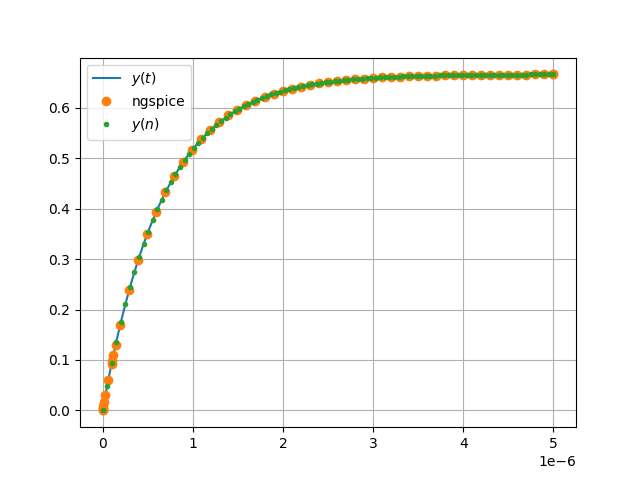
\includegraphics[width=\columnwidth]{./figures/4.7.png}
		\caption{Plots of $y(t)$ and $y(n)$}
		\label{fig-4.7}	
	\end{figure}
	
	\item Find $y(n)$ by solving the difference equation
	
	\solution 
	\begin{multline}
		y(n+1) \brak{1 + \frac{1}{2R_1C_0} + \frac{1}{2R_2C_0}} \\= y(n) \brak{1 - \frac{1}{2R_1C_0} - \frac{1}{2R_2C_0}} \\+ \frac{1}{R_2C_0}\brak{u(n)+u(n+1)}
	\end{multline}	
	
	For $n \ge 0$, $u(n) + u(n+1) = 2$
	\begin{multline}
		y(n+1) = y(n)\brak{\frac{1 - \frac{1}{2R_1C_0} - \frac{1}{2R_2C_0}}{1 + \frac{1}{2R_1C_0} + \frac{1}{2R_2C_0}}} \\+ \frac{\frac{2}{R_2C_0}}{1 + \frac{1}{2R_1C_0} + \frac{1}{2R_2C_0}}
	\end{multline}
	
	Let
	\begin{align}
		a &= \frac{1 - \frac{1}{2R_1C_0} - \frac{1}{2R_2C_0}}{1 + \frac{1}{2R_1C_0} + \frac{1}{2R_2C_0}} = -\frac{7.5\times10^5 -1}{7.5\times10^5 + 1}\\
		b &= \frac{\frac{2}{R_2C_0}}{1 + \frac{1}{2R_1C_0} + \frac{1}{2R_2C_0}} = \frac{10^6}{7.5\times10^5 + 1}
	\end{align}
	
	Therefore, the difference equation is
	\begin{align}
		y(n+1) &= ay(n) + b \\
		\implies y(n) &= ay(n-1) + b \\
		&= a(ay(n-2) + b) + b \\
		&= a^2(ay(n-3) + b) + b(1+a) 
	\end{align}
	
	On repeating this decomposition, we finally get
	\begin{align}
		y(n) &= a^ny(0) + b(1+a+\cdots+a^{n-1}) \\
		&= 0 + b\brak{\frac{1-a^n}{1-a}}	
	\end{align}
	\begin{multline}
		y(n) = \frac{10^6}{\cancel{7.5\times10^5 + 1}} \times \frac{\cancel{7.5\times10^5 + 1}}{2 \times 7.5\times10^5} \\ \times \brak{1 - \brak{-\frac{7.5\times10^5 -1}{7.5\times10^5 + 1}}^n }
	\end{multline}
	\begin{align}
		y(n) &= \frac{10}{15}\brak{1 - \brak{-\frac{7.5\times10^5 -1}{7.5\times10^5 + 1}}^n } && n \ge 0\\
		\therefore y(n) &= \frac{2}{3} \brak{1 - \brak{\frac{1-7.5\times10^5}{1+7.5\times10^5}}^n } u(n)
	\end{align}
	which is the same as what we obtained earlier
	
	
	\end{enumerate}
	\end{document}
